\section{Hagan Rowlenstino/1174040}
	\subsection{Soal 1}
	Bar :

	\lstinputlisting{src/6/1174040/Praktek/chap6_1174040_bar.py}

	\subsection{Soal 2}

	Scatter :

	\lstinputlisting{src/6/1174040/Praktek/chap6_1174040_scatter.py}

	\subsection{Soal 3}

	Pie :

	\lstinputlisting{src/6/1174040/Praktek/chap6_1174040_pie.py}

	\subsection{Soal 4}

	Plot :

	\lstinputlisting{src/6/1174040/Praktek/chap6_1174040_plot.py}

	\subsection{Penanganan Error}
	Error yang ditemukan yaitu ValueError. cara penanggulangan nya yatu dengan mengecek kembali panjang dan lebar subplotnya agar tidak kurang dari urutan yang kita buat.

	\lstinputlisting{src/6/1174040/Praktek/chap6_1174040_err.py}

\section{Faisal Najib Abdullah 1174042}
\subsection{Praktek}
\subsubsection{Soal No. 1}
\hfill \break
Buatlah librari fungsi (file terpisah/library dengan nama NPMbar.py) untuk plot dengan jumlah subplot adalah NPM mod 3 + 2!

\hfill \break
\textbf{Kode Program}

\lstinputlisting[caption = Kode program membuat fungsi Bar Plot menggunakan Matplotlib., firstline=1, lastline=21]{src/6/1174042/1174042_bar.py}

\hfill \break
\textbf{Hasil Compile}

\begin{figure}[H]
	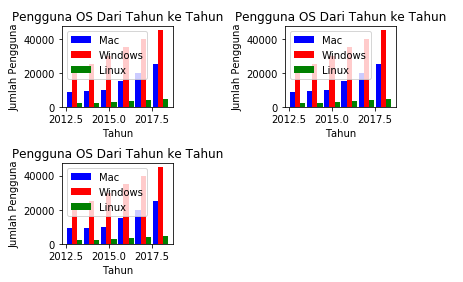
\includegraphics[width=12cm]{figures/6/1174042/p1.png}
	\centering
	\caption{Hasil compile membuat fungsi Bar Plot menggunakan Matplotlib.}
\end{figure}

\subsubsection{Soal No. 2}
\hfill \break
Buatlah librari fungsi (file terpisah/library dengan nama NPMscatter.py) untuk plot dengan jumlah subplot NPM mod 3 + 2!

\hfill \break
\textbf{Kode Program}

\lstinputlisting[caption = Kode program membuat fungsi Scatter Plot menggunakan Matplotlib., firstline=1, lastline=23]{src/6/1174042/1174042_scatter.py}

\hfill \break
\textbf{Hasil Compile}

\begin{figure}[H]
	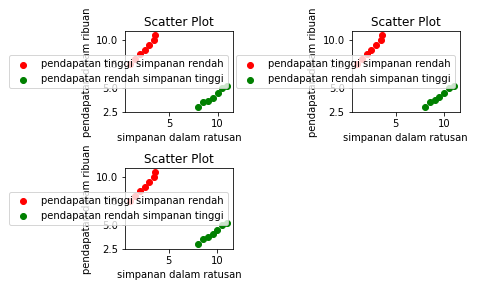
\includegraphics[width=12cm]{figures/6/1174042/p2.png}
	\centering
	\caption{Hasil compile membuat fungsi Scatter Plot menggunakan Matplotlib.}
\end{figure}

\subsubsection{Soal No. 3}
\hfill \break
Buatlah librari fungsi (file terpisah/library dengan nama NPMpie.py) untuk plot dengan jumlah subplot NPM mod 3 + 2!

\hfill \break
\textbf{Kode Program}

\lstinputlisting[caption = Kode program membuat fungsi Pie Plot menggunakan Matplotlib., firstline=1, lastline=23]{src/6/1174042/1174042_pie.py}

\hfill \break
\textbf{Hasil Compile}

\begin{figure}[H]
	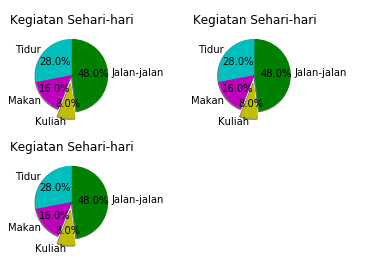
\includegraphics[width=12cm]{figures/6/1174042/p3.png}
	\centering
	\caption{Hasil compile membuat fungsi Pie Plot menggunakan Matplotlib.}
\end{figure}

\subsubsection{Soal No. 4}
\hfill \break
Buatlah librari fungsi (file terpisah/library dengan nama NPMplot.py) untuk plot dengan jumlah subplot NPM mod 3 + 2

\hfill \break
\textbf{Kode Program}

\lstinputlisting[caption = Kode program membuat fungsi Plot menggunakan Matplotlib., firstline=1, lastline=23]{src/6/1174042/1174042_plot.py}

\hfill \break
\textbf{Hasil Compile}

\begin{figure}[H]
	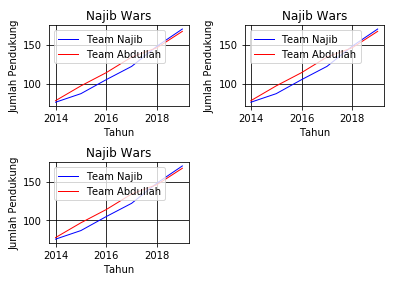
\includegraphics[width=12cm]{figures/6/1174042/p4.png}
	\centering
	\caption{Hasil compile membuat fungsi Plot menggunakan Matplotlib.}
\end{figure}


\subsection{Penanganan Error}
Tuliskan  peringatan  error  yang  didapat  dari  mengerjakan  praktek  keenam  ini, dan  jelaskan  cara  penanganan  error  tersebut. dan  Buatlah  satu  fungsi  yang menggunakan try except untuk menanggulangi error tersebut.

\hfill \break
Peringatan error di praktek kelima ini, yaitu:
\begin{itemize}
	\item Syntax Errors
	Syntax Errors adalah suatu keadaan saat kode python mengalami kesalahan penulisan. Solusinya adalah memperbaiki penulisan kode yang salah.
	
	\item Name Error
	NameError adalah exception yang terjadi saat kode melakukan eksekusi terhadap local name atau global name yang tidak terdefinisi. Solusinya adalah memastikan variabel atau function yang dipanggil ada atau tidak salah ketik.
	
	\item Type Error
	TypeError adalah exception yang akan terjadi apabila pada saat dilakukannya eksekusi terhadap suatu operasi atau fungsi dengan type object yang tidak sesuai. Solusi dari error ini adalah mengkoversi varibelnya sesuai dengan tipe data yang akan digunakan.
\end{itemize}
\hfill \break
Fungsi yang menggunakan try except untuk menanggulangi error.

\hfill \break
\textbf{Kode Program}

\lstinputlisting[caption = Kode program membuat fungsi penanganan error., firstline=161, lastline=178]{src/6/1174042/1174042.py}

\hfill \break
\textbf{Hasil Compile}

\section{Irvan Rizkiansyah/1174043}
	\subsection{Nomor 1}
	Histogram :
		\lstinputlisting{src/6/1174043/Praktek/chap6_1174043_hist.py}
	\subsection{Nomor 2}
	Scatter :
		\lstinputlisting{src/6/1174043/Praktek/chap6_1174043_scatter.py}
	\subsection{Nomor 3}
	Pie :
		\lstinputlisting{src/6/1174043/Praktek/chap6_1174043_pie.py}
	\subsection{Nomor 4}
	Plot :
		\lstinputlisting{src/6/1174043/Praktek/chap6_1174043_plot.py}
	\subsection{Penanganan Error}
		\lstinputlisting{src/6/1174043/Praktek/chap6_1174043_error.py}
	